\documentclass[conference]{IEEEtran}
\IEEEoverridecommandlockouts
\usepackage{cite}
\usepackage{amsmath,amssymb,amsfonts}
\usepackage{algorithmic}
\usepackage{graphicx}
\usepackage{textcomp}
\usepackage[table,xcdraw]{xcolor}
\usepackage{float}
\def\BibTeX{{\rm B\kern-.05em{\sc i\kern-.025em b}\kern-.08em
    T\kern-.1667em\lower.7ex\hbox{E}\kern-.125emX}}

\begin{document}

\title{The Exhaustion of IPv4 Address Space and the Transition to IPv6}

\author{
  \IEEEauthorblockN{Alexander Hoffmann}
  \IEEEauthorblockA{\textit{ECE Paris}\\
  Paris, France \\
  alexander.hoffmann@edu.ece.fr}
  \and
  \IEEEauthorblockN{Hugo Fougeres}
  \IEEEauthorblockA{\textit{ECE Paris}\\
  Paris, France \\
  hugo.fougeres@edu.ece.fr}
  \and
  \IEEEauthorblockN{Jeremy Roca}
  \IEEEauthorblockA{\textit{ECE Paris}\\
  Paris, France \\
  jeremy.roca@edu.ece.fr}
}

\maketitle

\section{Introduction}
At the beginning of networking, computer scientists were trying to determine the most efficient means of routing information so that it could be efficiently transmitted throughout the network. It was found that each connected computer maintains its own local address for the information it receives and that both the internetwork's most populous nodes (known as hubs) and the nodes connected to the most rural nodes do the same. Based on this information, and the IP version 4 address system was created. It uses 32 digital bits to represent addresses, generating a theoretical total limit of 4.3 billion addresses.

In May 2016 , International Internet Registration Authority (IARI), the authoritative organization for Internet numbering, declared the global Internet already fragmented. The IPv4 address space now supports only around 36,000 unique identifiers. At the rate of depletion, many, or even most, of the Internet's current home addresses could cease to exist within a decade. It is therefore not unrealistic to expect many existing IP-based applications and services to disappear from the internet at some time in the foreseeable future. It is likely that the first to go will be file sharing, but it is equally possible that other notable Internet-based services, such as online games, forums, instant messaging, and backup, will go in that order. Certain "workarounds" have been proposed to try to keep the web alive, such as re-using one-time addresses, mixing address pairs, and distributed denial of service. But the picture is grim.

Due to degradation in the availability of new IPv4 addresses, some of the community switched to IPv6. New trends in Internet innovation and increased usage of broadband make IPv6 an attractive choice. The most recent public audit, however, found that the Internet's IPv6 address space is still shrinking. In 2008, the Internet reached a global peak of IPv6 addresses.

This paper discusses the depletion of IPv4 addresses. The paper also reviews replacement strategies. Currently, IPv6 is the most widely cited replacement candidate for IPv4. This document analyses IPv6 as an example replacement and goes over technical and security components of IPv6.

\section{Internet Addressing}
The Internet Protocol (IP) is the dominant network protocol upon which many applications run.  This involves everything from Web browsing, to the stability of data communication, to the bandwidth efficient nature of broadband communications. There are many communication protocols, the most common of which are TCP and UDP. All of these protocols in turn use IP to translate between traffic types. Each Internet protocol is optimized for a particular purpose, such as routing packets and transferring data from point to point.

IPv4  was created in the early 1970s as an Internet Protocol that ran over the Department of Defense/US military, allowing secure messages between US Army "black sites". It offers a uniform solution to the problem of identifying hosts that should be allocated resources and to problems associated with timing and address inconsistencies. IPv4 addresses are 16-bit integers, and are generally 128 bits wide. For instance, an IP address can consist of eight characters (like e.g. 192.168.1.100). Each Internet service provider (ISP) has its own "Network Address Translation" (NAT) software.  It translates each IP address in the public Internet to its private.

In the late 1990s, however, someone suggested an expansion of the IP protocol. IPv6  was created in 2000, with over 4 million people at present using it, to replace IPv4. From a security point of view, IPv6 is considered to be far more secure than IPv4 and runs with a small amount of overhead and no external dependency for critical services such as e-mail. IPv6 makes possible new functionality, such as distributing source addresses and addressing requests within multicast groups (i.e. broadcasts), delivering many more addresses in more contexts, and enabling network topologies to be defined in terms of many subnets instead of a single large address block.

Internet routers route by breaking each IP address into a network number and a host number on that network. Each host on a network is assigned a number, and the router then puts those hosts together to form a single network that can be given a specific IP address. Routing protocols are clever: they figure out how to translate between network numbers and hosts, while keeping the IP address.

\section{IPv4 Address Shortage}
Internet growth is inextricably related to the expansion of IPv4 Address Space consumption. For nearly a decade, the Internet has grown rapidly across the world, and space limitations for the 32-bit IPv4 address have become severe. The increasing demand for IPv4 infrastructure will increase the cost of procuring and managing IPv4 address space, and give Internet Service Providers an incentive to procure and offer and offer more IPv4 capacity to their customers. Reports about the date at which the IPv4 address space will be exhausted vary. Fig \ref{summary} represents a summary of some reports.
\begin{figure}
\begin{table}[H]
\centering
\begin{tabular}{|l|c|c|c|c|}
\hline
\rowcolor[HTML]{3166FF} 
\multicolumn{1}{|c|}{\cellcolor[HTML]{3166FF}Document}                                                                              & Issued                                              & Author                                                  & IANA                                                & RIR                                                 \\ \hline
\begin{tabular}[c]{@{}l@{}}The ISP Column\\ (How long have we \\ got?)\end{tabular}                                                 & \begin{tabular}[c]{@{}c@{}}Jul.\\ 2003\end{tabular} & \begin{tabular}[c]{@{}c@{}}Geoff \\ Huston\end{tabular} & 2021                                                & 2022                                                \\ \hline
\begin{tabular}[c]{@{}l@{}}IPv4 Address Report\\ (Potaroo)\end{tabular}                                                             & \begin{tabular}[c]{@{}c@{}}Dec.\\ 2005\end{tabular} & \begin{tabular}[c]{@{}c@{}}Geoff \\ Huston\end{tabular} & \begin{tabular}[c]{@{}c@{}}Jan.\\ 2013\end{tabular} & \begin{tabular}[c]{@{}c@{}}Jan.\\ 2016\end{tabular} \\ \hline
\begin{tabular}[c]{@{}l@{}}Internet Protocol\\ Journal \\ (A Pragmatic Report \\ on IPv4 Address \\ Space Consumption)\end{tabular} & \begin{tabular}[c]{@{}c@{}}Sep.\\ 2005\end{tabular} & \begin{tabular}[c]{@{}c@{}}Tony\\ Hain\end{tabular}     & 2009                                                & 2016                                                \\ \hline
\begin{tabular}[c]{@{}l@{}}The ISP Column\\ (Numerology)\end{tabular}                                                               & \begin{tabular}[c]{@{}c@{}}Nov.\\ 2005\end{tabular} & \begin{tabular}[c]{@{}c@{}}Geoff \\ Huston\end{tabular} & \begin{tabular}[c]{@{}c@{}}Jan.\\ 2012\end{tabular} & \begin{tabular}[c]{@{}c@{}}Mar.\\ 2013\end{tabular} \\ \hline
\end{tabular}
\end{table}
\caption{Summary of IPv4 exhaustion reports}
\label{summary}
\end{figure}

On 31 January 2011, the last two unreserved IANA /8 address blocks were allocated to APNIC according to RIR request procedures. This event can be observed on Fig \ref{ipv4-exhaust}.
\begin{figure}[htbp]
\centerline{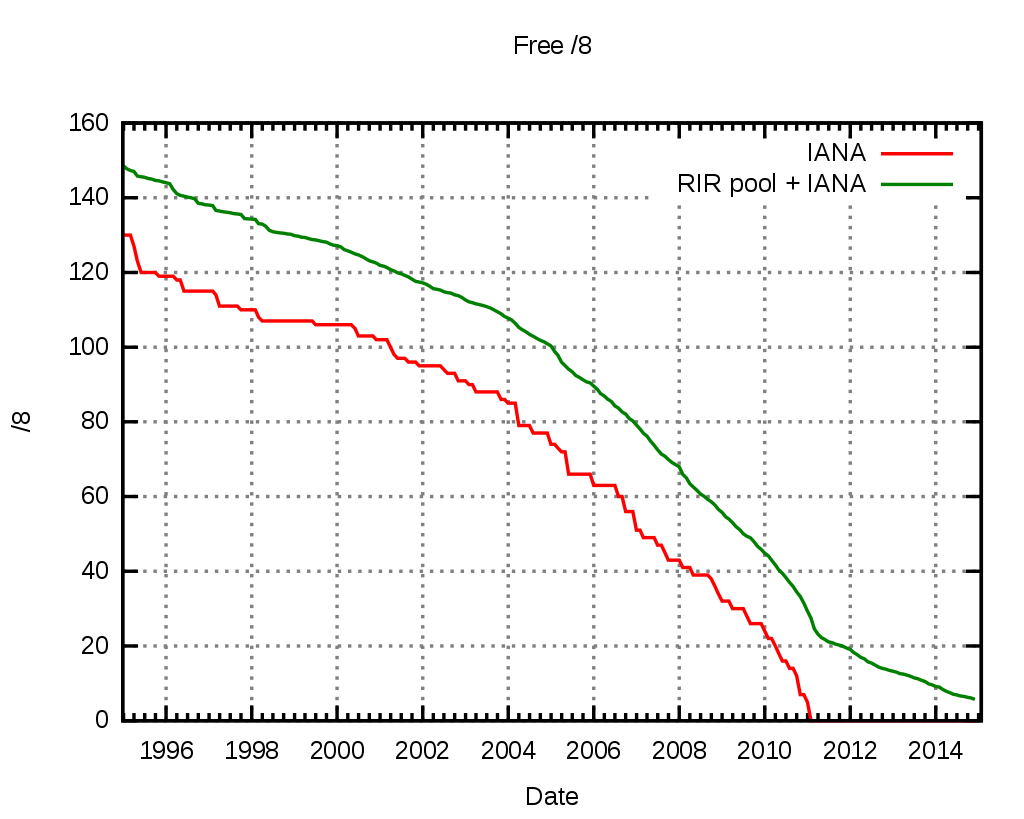
\includegraphics[scale=0.25]{resources/ipv4-exhaust.png}}
\caption{Exhaustion of IPv4 addresses since 1995}
\label{ipv4-exhaust}
\end{figure}
The IPv4 address space shortage had already been expected as early as 1990. Still, Fig \ref{summary} shows how complex it was to predict the actual date of exhaustion.

\end{document}
